\section{Testbed Setup, Deployment and Results}
\label{ch:Physical Network}

To show the gains of leveraging heterogeneity in WSNs, a testbed deployment was created and run. Test runs
using both HCCP and LEACH as the network clustering protocol were created, run and compared. 

\subsection{Building HCCP with 802.15.4}


The goal of HCCP is to intelligently cluster motes in Wireless Sensor Networks, not to 
create a new wireless standard. HCCP works as a middleware layer between the 
mote's application and the wireless radio that is using some wireless protocol, 
such as Bluetooth, ANT radios, or even WIFI (802.11). The
network protocol used in the testbed deployment was 802.15.4.

Building on top of 802.15.4 requires that the protocol's requirements are met. 
A basic packet in 802.15.4 is constructed using several segments that
have information in well-defined places, as seen in Table~\ref{fig:eightOhTwo}.
The physical layer header preamble is handled by the hardware and is outside the scope
of this work. It is assumed that the preamble is functioning properly, and no changes need to be made
to it for the support of HCCP.

The bytes following the physical layer preamble are the Media Access Control (MAC) layer
header bytes. The bytes in the header are well-defined by the 802.15.4 protocol,
with each byte given a special meaning in the header.  
The first two bytes are the Frame Control Field (FCF), which can be seen in Table~\ref{fig:eightOhTwo},
that tell the packet parser
what to expect in the rest of the packet. The FCF details values which affect
how long the packet header will be such as whether
the security is enabled, and which type of MAC addresses the packet header
contains. 

The next byte is the packet sequence number, which is a value that gets incremented for
every packet the sending mote sends. It is used to recreate data that is split across multiple packets
that are being sent to the receiving mote. In the testbed deployment, data is assumed to be 
contained within one packet. The sequence number of the packets is therefore irrelevant, but can not be
left out without violating the guidelines described by the 802.15.4 standard.


%\begin{figure}[htbp]
%	\centering
%		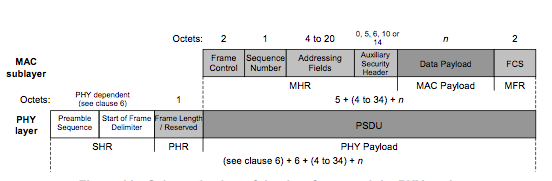
\includegraphics[width=6.5in]{images/protocol/8oh2.png}
%	\caption{Breakdown of data packets in 802.15.4.~\cite{zigbee}}
%	\label{fig:eightOhTwo}
%\end{figure}
%\begin{figure}[htbp]
%	\centering
%		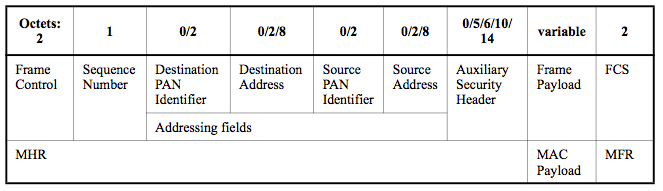
\includegraphics[width=5in]{images/protocol/MacFrame.png}
%	\caption{General 802.15.4 frames, as shown in the 802.15.4 standards document~\cite{zigbee}.}
%	\label{fig:images_protocol_MacFrame}
%\end{figure}


\begin{table}[ht]
	\centering
	\begin{scriptsizetabular}{|c|c|c|c|c|c|c|}

      \hline 
      Octets:  &          &           &              &          &        &  \\
      variable & 2        &  1        & 4-20         &  0-14    & n      &  2\\
      \hline 
      Preamable & Frame    & Sequence  & Addressing  & Security & Data   &  Checksum\\
      Sequence & Control  & Number    & Fields      & Header   & Payload &  \\ 
      \hline
    \end{scriptsizetabular}
    \caption{Breakdown of data packets in 802.15.4. Adapted from~\cite{zigbee}.}
    \label{fig:eightOhTwo}
\end{table}


% m{width}
%\begin{table}[ht]
%	\centering
%	\begin{scriptsizetabular}{|c|c|c|c|c|c|c|c|}
%		\hline
%		Frame  & Sequence & Destination & Source & Auxiliary & HCCP Packet & HCCP Packet & Checksum  \\
%		Control  & Number & Address & Address & Security Header & Type & Payload &  \\
%		\hline 
%	\end{scriptsizetabular}
%	\caption{Customized 802.15.4 packets for use in HCCP with more detail.}
%	\label{tab:Mypackets}
%\end{table}
\begin{table}[ht]
	\centering
	\begin{scriptsizetabular}{|m{1cm}|m{1.35cm}|m{1.75cm}|m{1.35cm}|m{1.5cm}|m{1.25cm}|m{1.80cm}|m{1.5cm}|}
		\hline
		Frame Control & Sequence Number & Destination Address & Source Address & Auxiliary Security Header & HCCP Packet Type & HCCP Packet Payload & Checksum  \\
		\hline 
	\end{scriptsizetabular}
	\caption{Customized 802.15.4 packets for use in HCCP with more detail.}
	\label{tab:Mypackets}
\end{table}




Following the sequence number is the addressing field, which can be 4-20 bytes. The range is due to the 
way that 802.15.4 addresses can be specified. 802.15.4 has 20 byte addresses that are designed to be globally unique identifiers,
but can also use 4 byte addresses to create lightweight packets. When using the 4 byte addresses there is a good chance that 
two motes in the network could have the same address. This causes the tradeoff of reliability and understandably of data versus
the per packet cost to send a message in the network. There is both a source and destination address specified in the addressing field.

An optional security field follows the sequence number. This field could be used to encrypt the data in the packet,
but it not used in the testbed deployment. HCCP can be used with encryption using this field with little or no modifications
to the HCCP protocol.

Finally, the data payload for an 804.15.4 packet is where all the HCCP logic is added. HCCP divides up the 
data section of the packet into more well-known fields, much like the creators of 802.15.4 have done. 
HCCP divides the data section in to 8 bits for packet type, and the remainder is the packet data.
The custom HCCP packet format is shown in Table~\ref{tab:Mypackets}.  The
The HCCP values for the HCCP Packet Type field are as follows:

\begin{enumerate}
	\item \textbf{Clusterhead Candidacy Announcement} - {\tt 0x0} - The sender of this message is going to be a clusterhead candidate.
	\item \textbf{Clusterhead Announcements} - {\tt 0x1} - The sender of this message is a clusterhead. Following the HCCP header is the mote's ID.
	\item \textbf{Join Cluster} - {\tt 0x2} - The sender of this message wants to join the cluster of the recipient. The mote that has the address in the addressing field is the mote 
	it will follow. The clusterhead that is the recipient will use the `from' address as the ID of its new clustermote.
	\item \textbf{TDMA Schedule} - {\tt 0x3} - A broadcast message to all surrounding motes with the TDMA schedule the 
	clustermotes will be following. A sample TDMA schedule
	can be seen in Table~\ref{tab:tdma}. \begin{table}[ht]
		\centering
		\begin{tabular}{|c|c|c|c|c|c|c|c|}
			\hline
			Packet  &  Runtime for  & First ID & Second ID &  ... & nth ID\\
			Type &  each Mote (s or ms) & \& Delay & \& Delay &  & \& Delay \\
			\hline
			{\tt 0x3} & 20 & 12:20 & 18:40 & ... & 88:70\\
			\hline
		\end{tabular}
		\caption{Sample TDMA schedule as sent by the clusterhead to its clustermotes.}
	\label{tab:tdma}
\end{table}
	
	\item \textbf{Data Packet} - {\tt 0x4} - Messages sent from clustermotes to their clusterhead. $n$ data bytes will follow the type field.
	\item \textbf{Roundtable Discussion Packet} - There are a few well-defined packets that can be sent during a Roundtable Discussion. To save in the packets, they 
	can share the type field with the other well-defined packets, or can be assigned type values of their own.
	\begin{enumerate}
		\item \textbf{Clusterhead Opt-out} - {\tt 0x5} - Clusterhead can quit if there are multiple iterations of the 
		HCCP schedule. 
		\item \textbf{Roundtable Clusterhead Announcement} - {\tt 0x6} - a replacement clusterhead if an existing clusterhead opts out.
	\end{enumerate}
	\item \textbf{Other} - {\tt 0x8} - If any packets are defined for a customization of HCCP, this value can be used. An instance where other packets could be used
	is during the Roundtable Discussion, if the motes need to share some other information. In the testbed deployment, routing information is shared using the
	other packet type during the Roundtable Discussion time. The contents following the HCCP header are at the discretion of the network administrator.
\end{enumerate}

After the HCCP packet type field is the HCCP packet data field which contains the 
packet payload. After that the 802.15.4 checksum follows to make the packet 802.15.4 compliant.



\subsection{Description of Testbed Motes}
\label{ch:motes}

To create a heterogeneous WSN, motes from multiple vendors 
were selected for the experimental WSNs. The motes selected 
have different radios, run different operating systems and
have differing capabilities. Below is a description of the
motes used for the experiments, the capabilities of the motes,
the modifications that could be possible to increase heterogeneity and the modifications made to them.


\subsubsection {Sun Microsystems SunSPOT}
 
	Sun Microsystems Labs~\cite{sunspot} saw the need for easily programmable
	motes with solid form-factor and simple tools to use. 
	SunSPOT stands for `Sun Microsystems Small Programmable Object Technology', which 
	is designed to be simple to both program and deploy.
	Sun had already 
	created a version of Java to run on mobile phones called Java 2 Micro Edition (J2ME)~\cite{j2me}.
	Sun used this code base for a starting point for the SunSPOT programming interface. 


	The SunSPOTs are sold in boxes with 2 motes called ``free-range'' motes seen in Figure~\ref{fig:images_motes_sunspot1}, and 
	one base station mote, as seen in Figure~\ref{fig:images_motes_sunspotandBS}. The free range motes are complete with a 
	rechargeable battery
	that charges from USB, a CC2420 radio, a number of sensors and LEDs for the programmer
	to use. The free range SunSPOTs are divided into 2 boards, as seen in Figure~\ref{fig:images_motes_sunspot2}. The top board is the board visible
	on the top of the SunSPOT, which is the sensor board that holds all the 
	sensors, buttons and LEDS. The second board is the main board that hosts the microcontroller and the radio.
	The base station SunSPOTs share the same main board as the free range SunSPOTs, but do not have
	a rechargeable battery or a sensor board. The common main board is convenient, as the radio code
	can be shared between the both the free-range motes, and the base station.
	
	 \begin{figure}[htbp]
	 	\centering
	 		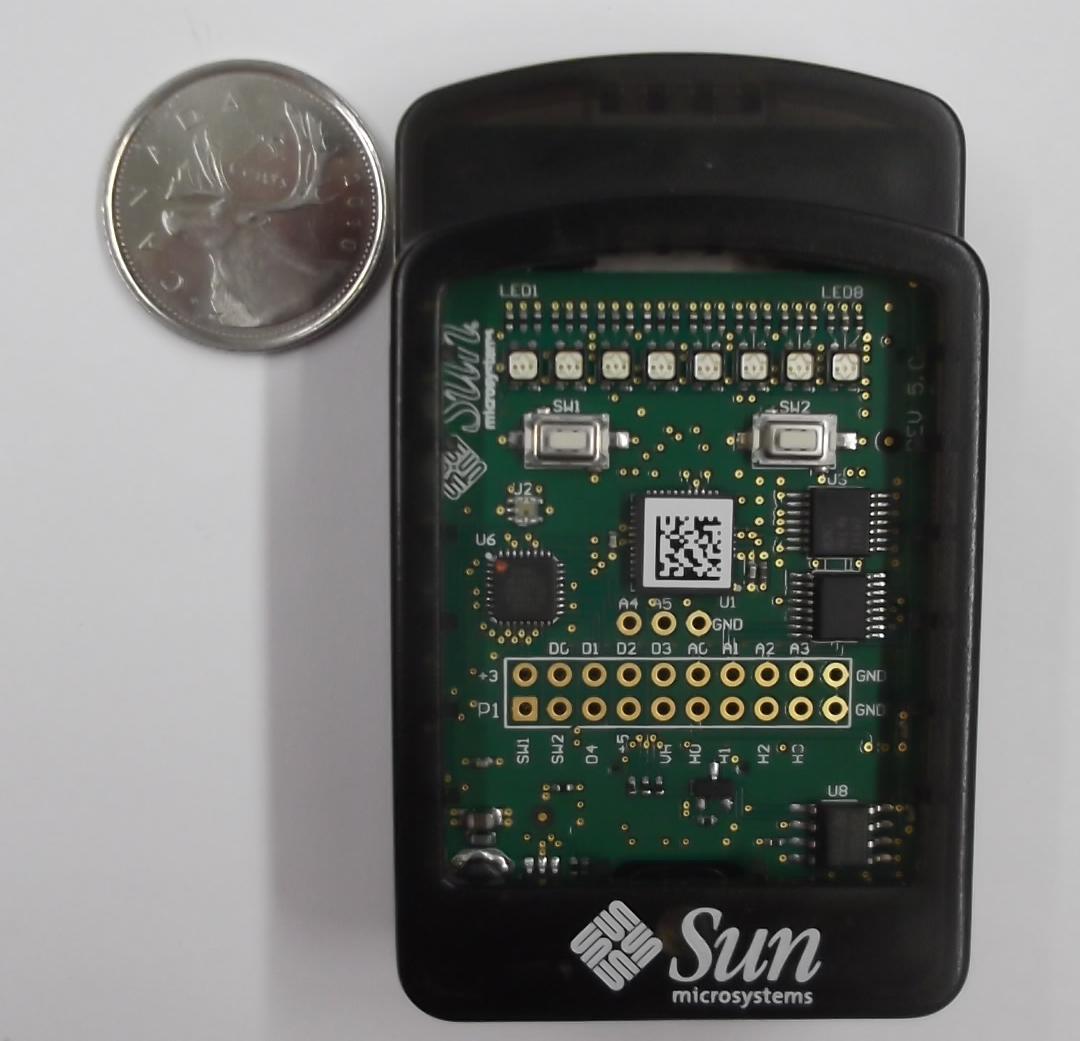
\includegraphics[height=3in]{images/motes/sunspot1.jpg}
	 	\caption{The Sun Microsystems SunSPOT.}
	 	\label{fig:images_motes_sunspot1}
	 \end{figure}
	\begin{figure}[htbp]
	 	\centering
	 		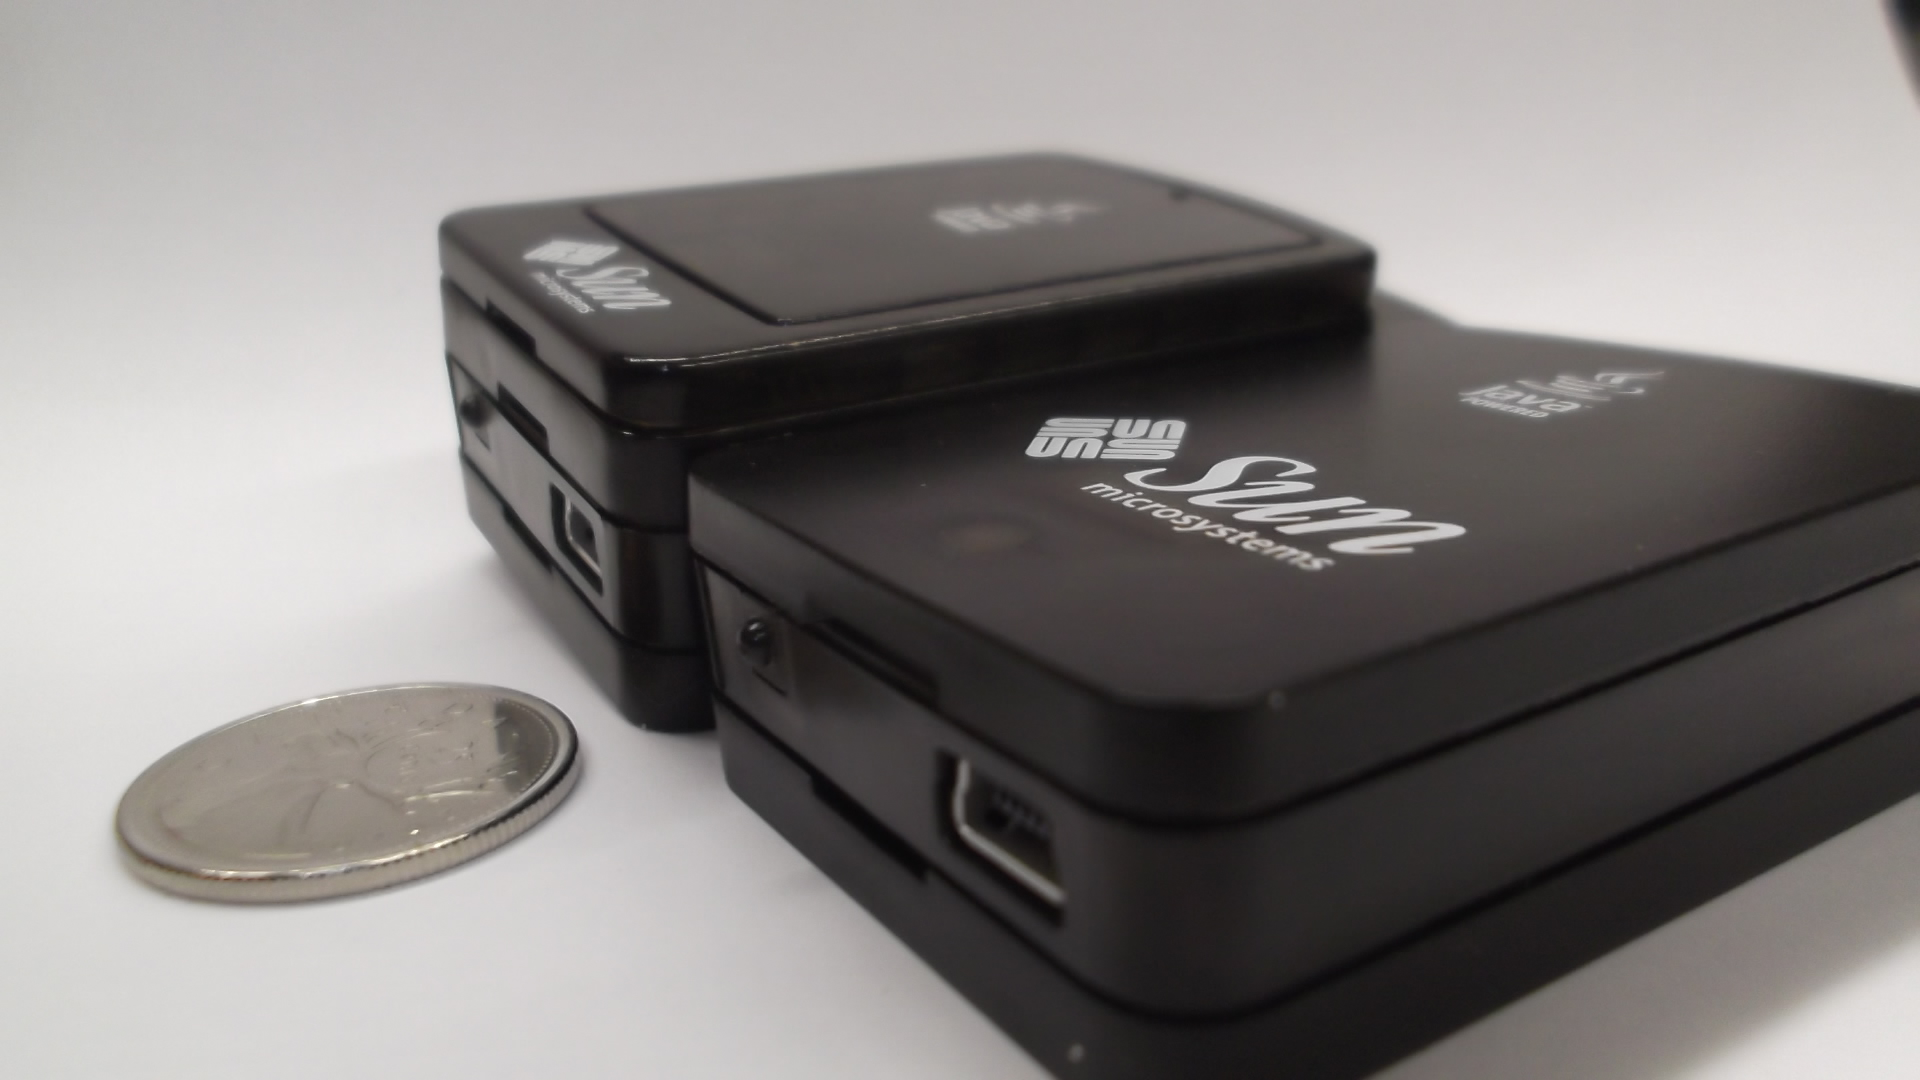
\includegraphics[height=3in]{images/motes/spotBSandMote.jpg}
	 	\caption{A SunSPOT free-range mote and SunSPOT base station.}
	 	\label{fig:images_motes_sunspotandBS}
	 \end{figure}
	 \begin{figure}[htbp]
	 	\centering
	 		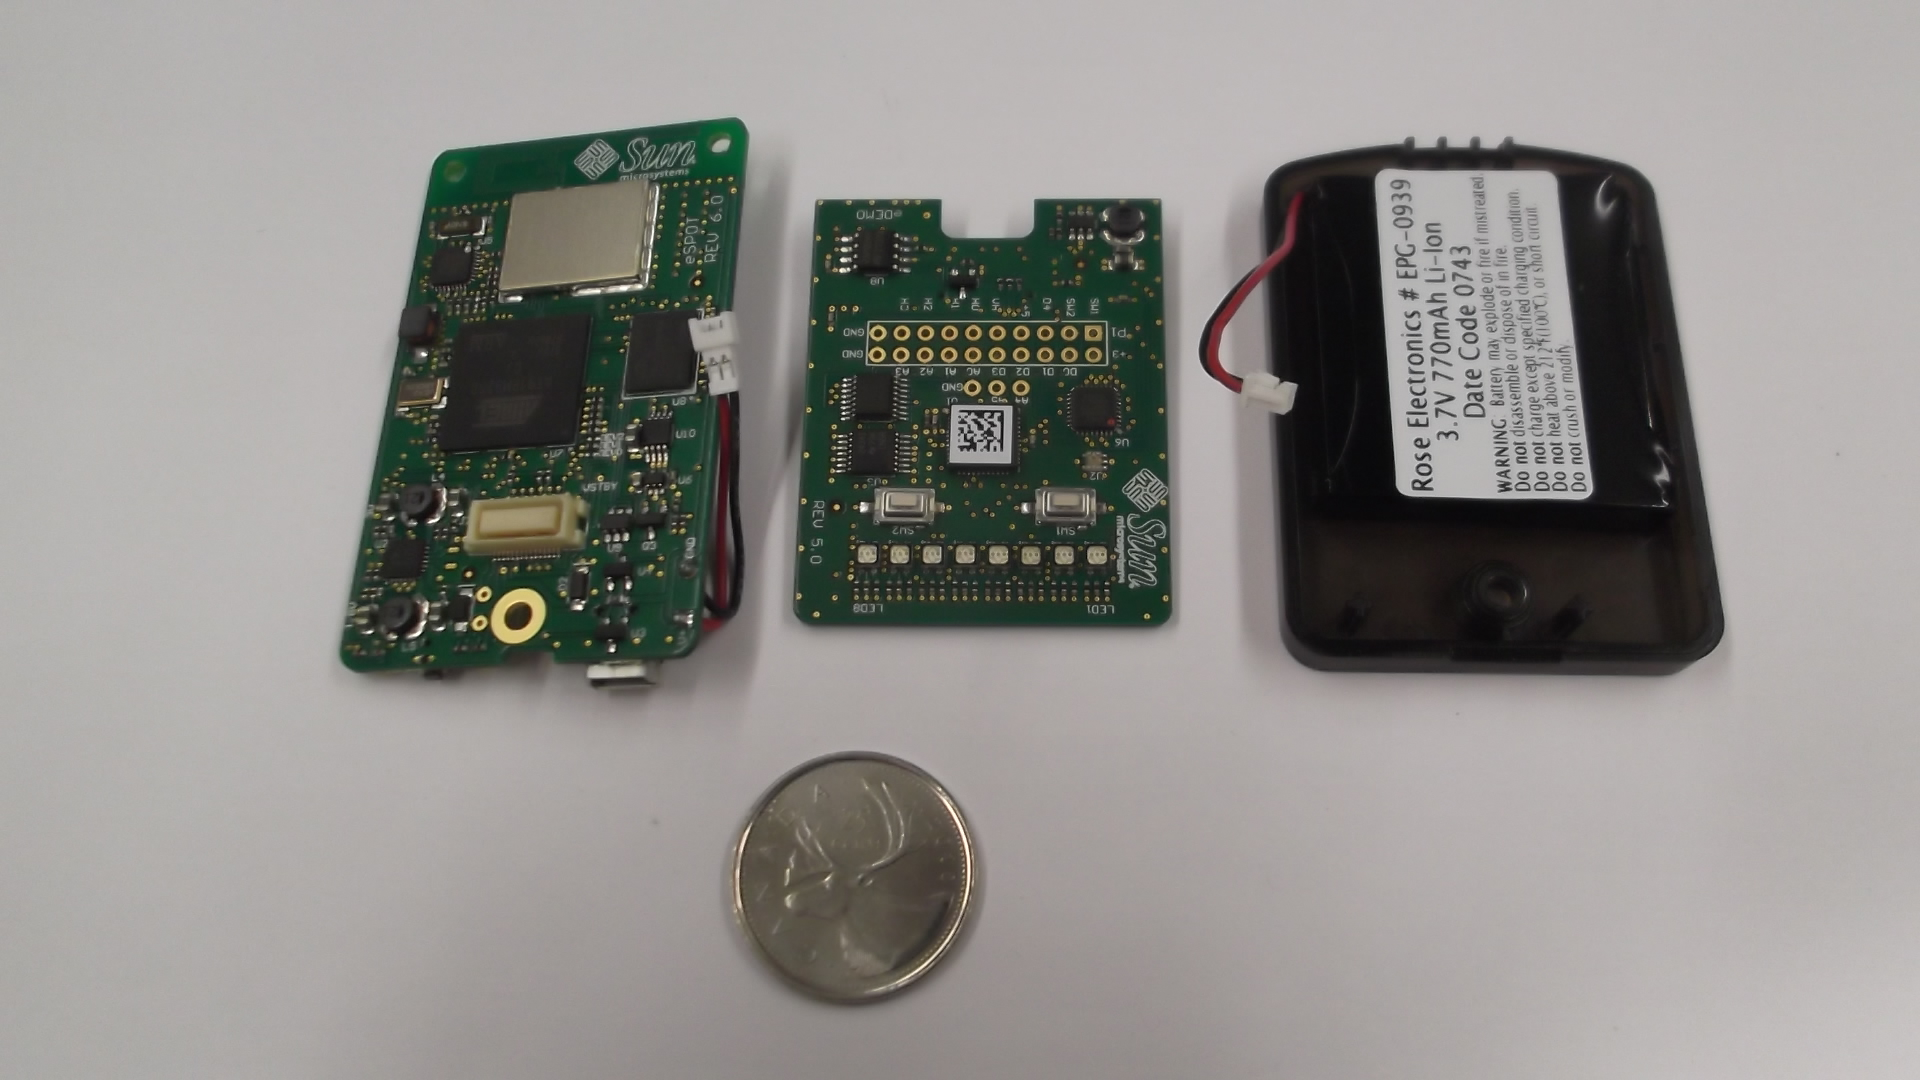
\includegraphics[height=3in]{images/motes/sunspot2.jpg}
	 	\caption{A SunSPOT taken apart to view the components in the casing.}
	 	\label{fig:images_motes_sunspot2}
	 \end{figure}
 
\paragraph{\emph{Possible Modifications to the SunSPOTs.}}
	The rechargeable battery the SunSPOTs ship with is small and does not hold 
	enough energy to power the SunSPOT for a long period of time. A simple modification is
	to remove the back of the SunSPOT, replacing the battery with any other power source providing 
	up to 4.9 volts as stated in the SunSPOT developer's manual~\cite{sunspotmanual}. 
	This could be done with 3 AA batteries, which would provide much more available energy.
	
\paragraph{\emph{Uses for the SunSPOT in a Heterogeneous WSN.}}
	The base station the SunSPOTs ship with makes a very convenient base station for a 
	WSN. The radio code developed for the free range SunSPOTs can be used on the base station
	while it is connected to a computer. The base station is designed to run with
	Java code developed using the SunSPOT suite developed for the SunSPOT, and
	the base station can be easily accessed via a Java program. The program running the 
	base station can then log the data to a database, or post it to a website to make the 
	data collected by the WSN available world-wide immediately.
	
	The base station could also be used to make an entire computer a mote.
	That is to say, the base station could be connected to a computer but not act 
	as a sink. This would allow the mote to have nearly unlimited power and memory resources, 
	making it an ideal routing mote.

	\begin{figure}[tbh]
		\centering
			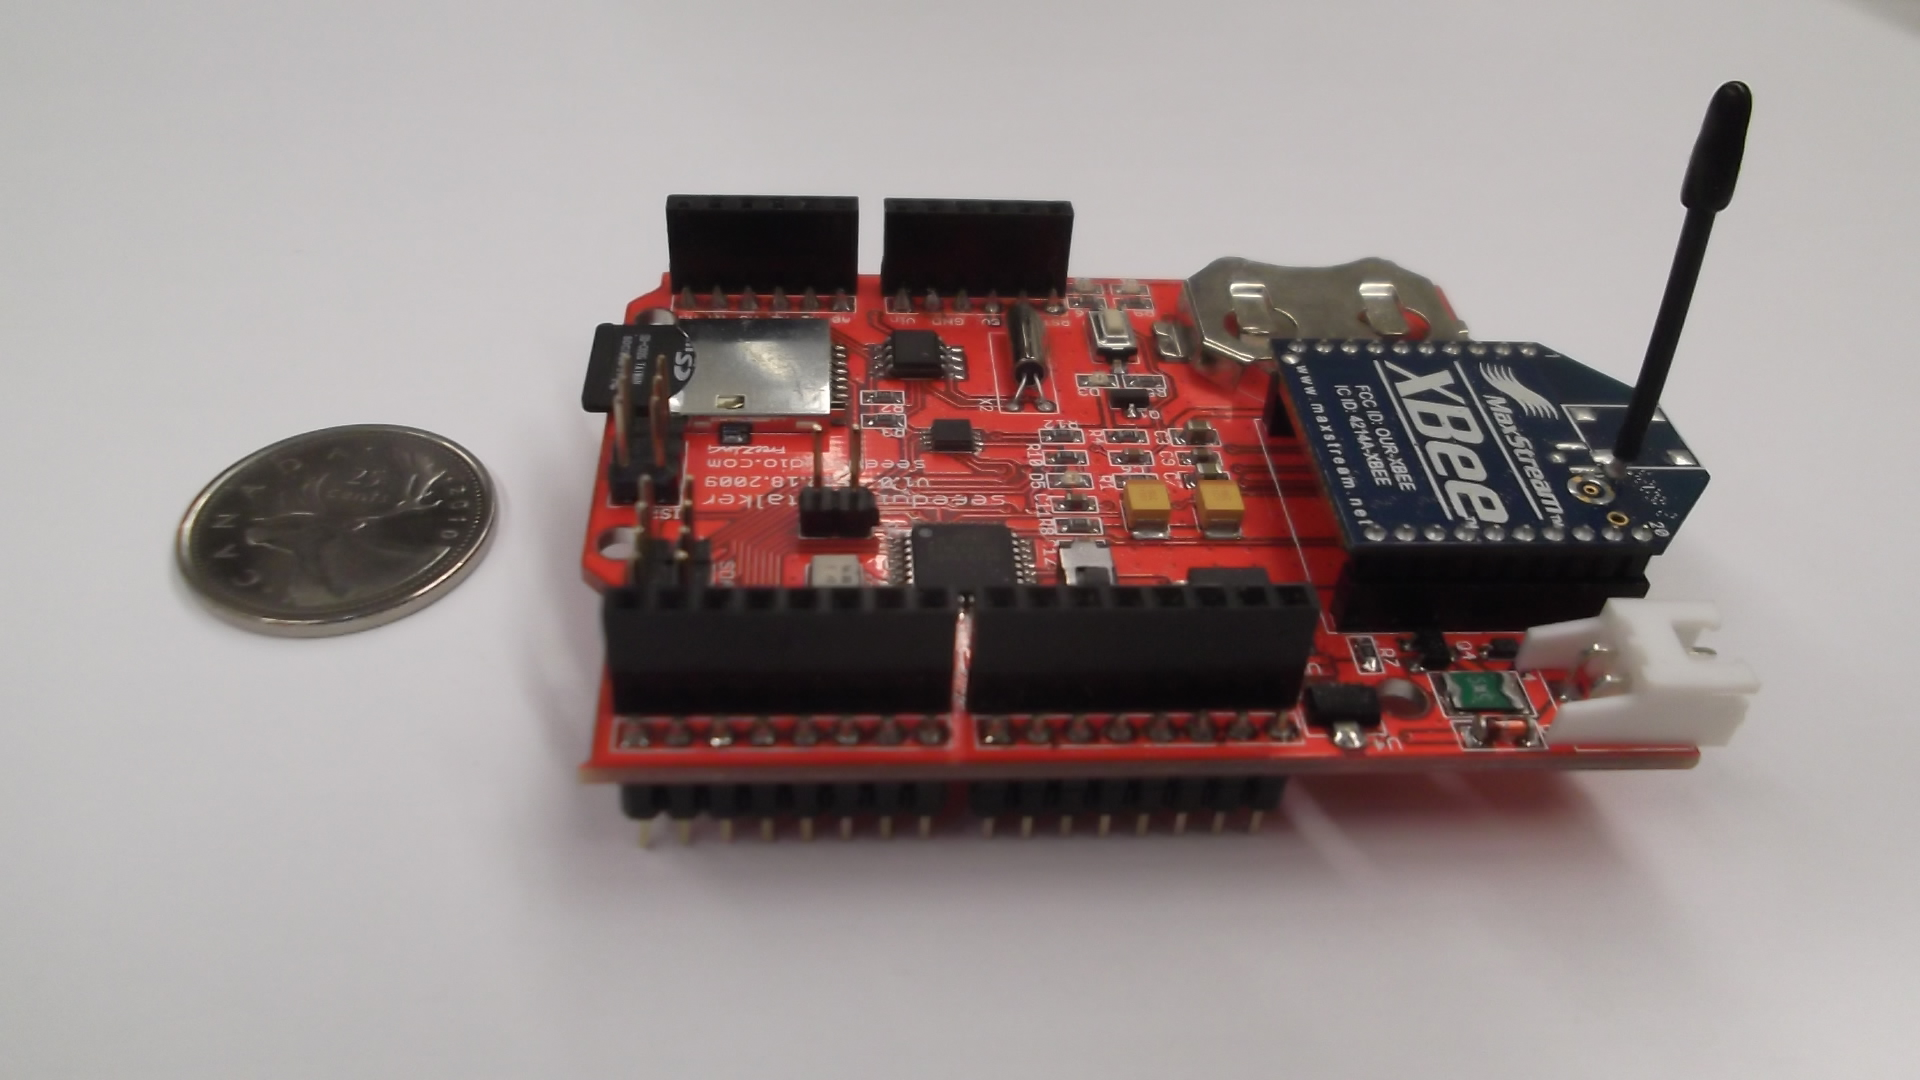
\includegraphics[height=3in]{images/motes/stalkerXbee1.jpg}
		\caption{Seeeduino Stalker with XBee port exposed.}
		\label{fig:images_motes_stalkerXbee1}
	\end{figure}

\subsubsection {Seeeduino Stalker and Arduino Technology}
	Seeed Studios~\cite{seedstalker} is a developer and retailer of microcontrollers online, 
	specializing in Arduino-compatible microcontrollers. One of the products they provide
	is a mote called the Seeeduino Stalker. The Stalker is a microcontroller based on the 
	Arduino design~\cite{arduino}, using a compatible processor and standard Arduino pin layouts.
	As seen in Figure~\ref{fig:images_motes_stalkerXbee1} the
	Stalker has an onboard battery, and logging capabilities, using MicroSD cards to log to.
	The Stalker does not ship with a built-in radio, but makes an XBee compatible slot available. 
	To allow the Stalker to communicate with the other motes, we chose the XBee Series 1 
	modules - which communicate using the 802.15.4 standard~\cite{zigbee}.
	
	The Stalker does not have any native sensing abilities, but can be configured to use
	either Arduino-compatible shields (which attach to the female pin headers on the board 
	to provide some service). This makes the Stalker ideal for creating highly customized
	motes. The Stalker could be configured to have no sensors to make a low-power routing
	mote with the ability to log large amounts of data on its MicroSD card. Or, can be configured
	to use a variety of sensors and be a specialized sensor mote.
	
	A problem does arise with the Stalker's battery power. The Stalker is sold with a port to 
	use a `button battery', as seen in Figure~\ref{fig:images_motes_stalkerXbee1}. More power is 
	very desirable, so the Seeeduino Stalker motes will need to be fitted with a larger battery supply before
	it could be used as a useful mote.  The Stalker is sold with a port to plug in an external 
	power supply, so this is not a large problem.
	
	A major problem with the Stalker is the CPU it uses. The CPU has very limited program space. 
	The code developed frequently overran the size of the program space, causing the 
	mote to crash. Due to this, a minimal installation of Contiki OS has been created to 
	allow the Stalker to work in the network with limited capabilities. The Stalker
	can only participate in the network as a clustermote, not as a Clusterhead.
	
	Another Arduino mote was made for the network. The Arduino Duemilanove is a more powerful Arduino with 
	more memory and fewer built-on features. The Duemilanove required an extension called 
	a shield to allow the board to use a radio, as seen in Figures~\ref{fig:images_motes_arduinoUnstack} 
	and~\ref{fig:images_motes_arduinoStack}. By adding a radio extension, the Arduino gains 
	the ability to send data over an 802.15.4 network, but does not replicate the logging ability 
	the Stalker has. 
	

	\begin{figure}[\begin{figure}[htp]
		\centering
			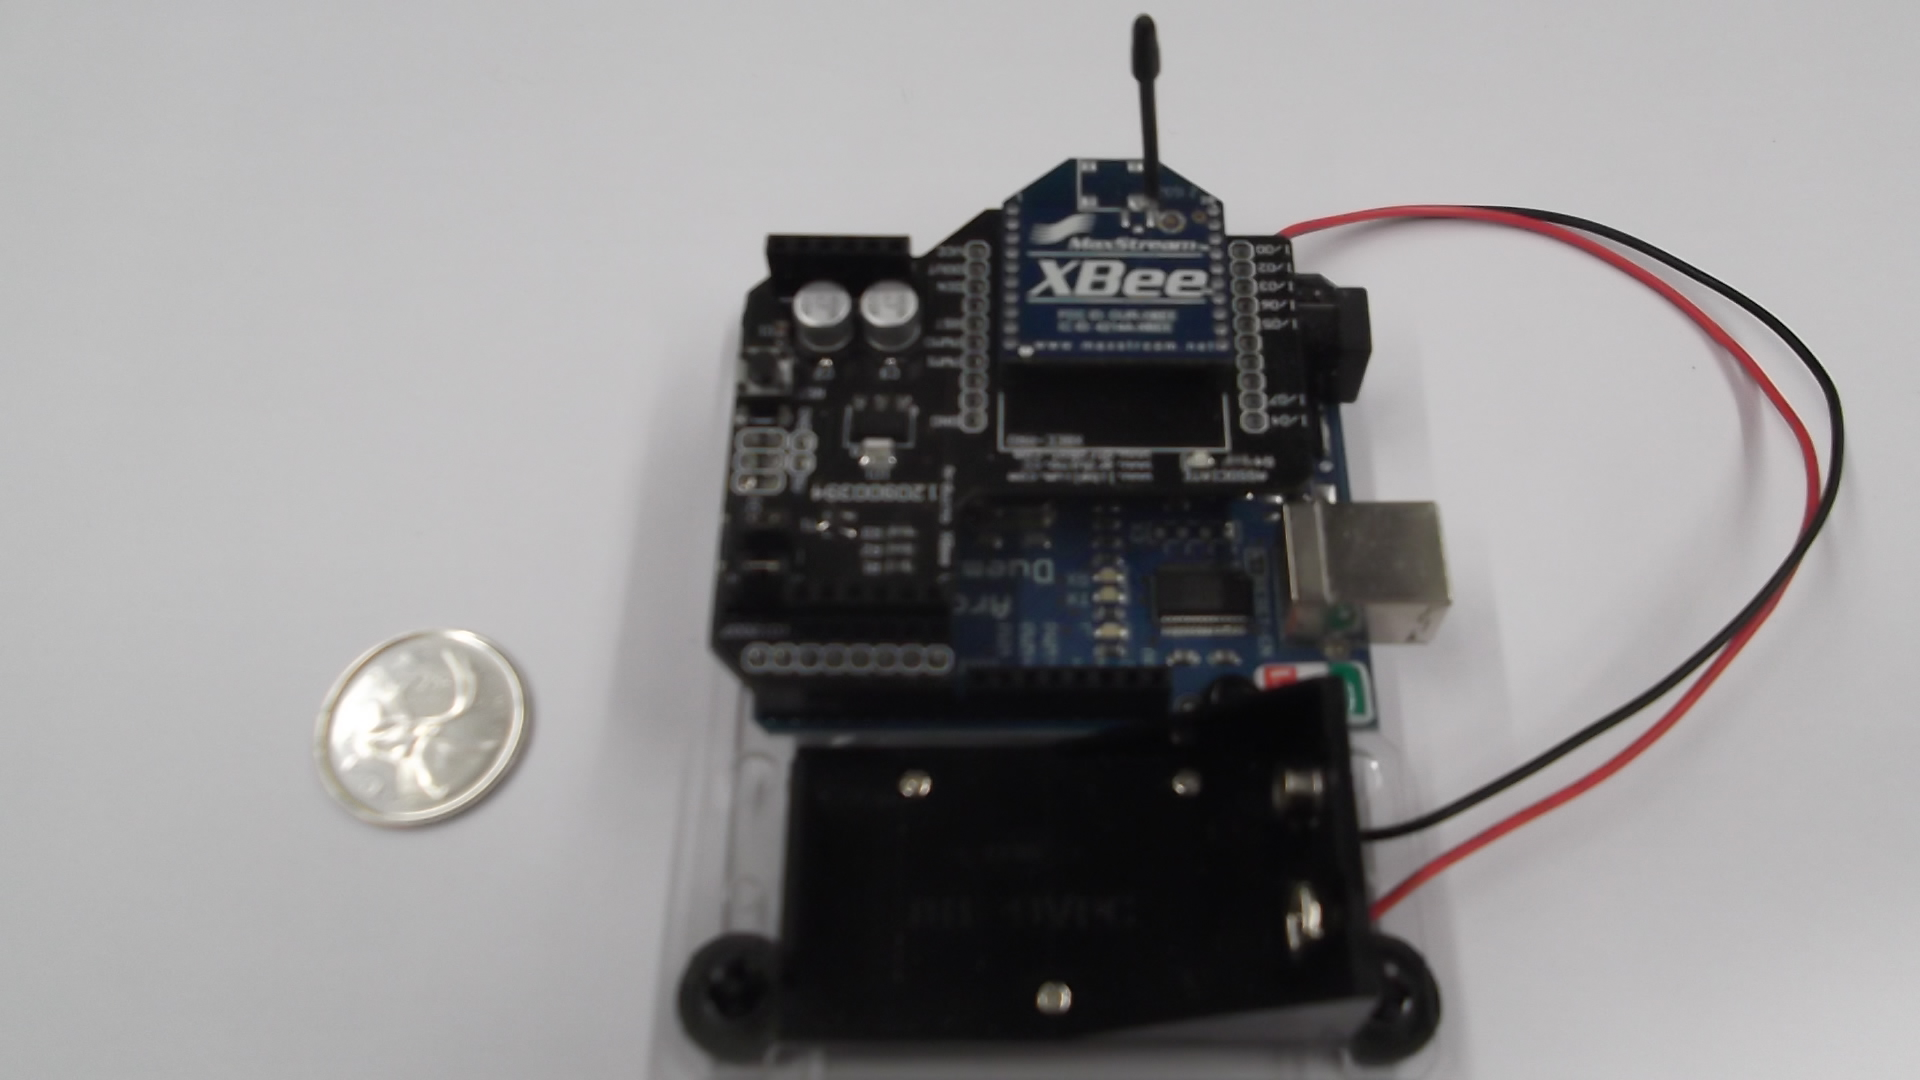
\includegraphics[height=3in]{images/motes/arduinoStack.jpg}
		\caption{An Arduino Duemilanove turned into a mote using the XBee Shield and an XBee radio.}
		\label{fig:images_motes_arduinoUnstack}
	\end{figure}
	
	\begin{figure}[\begin{figure}[htp]
		\centering
			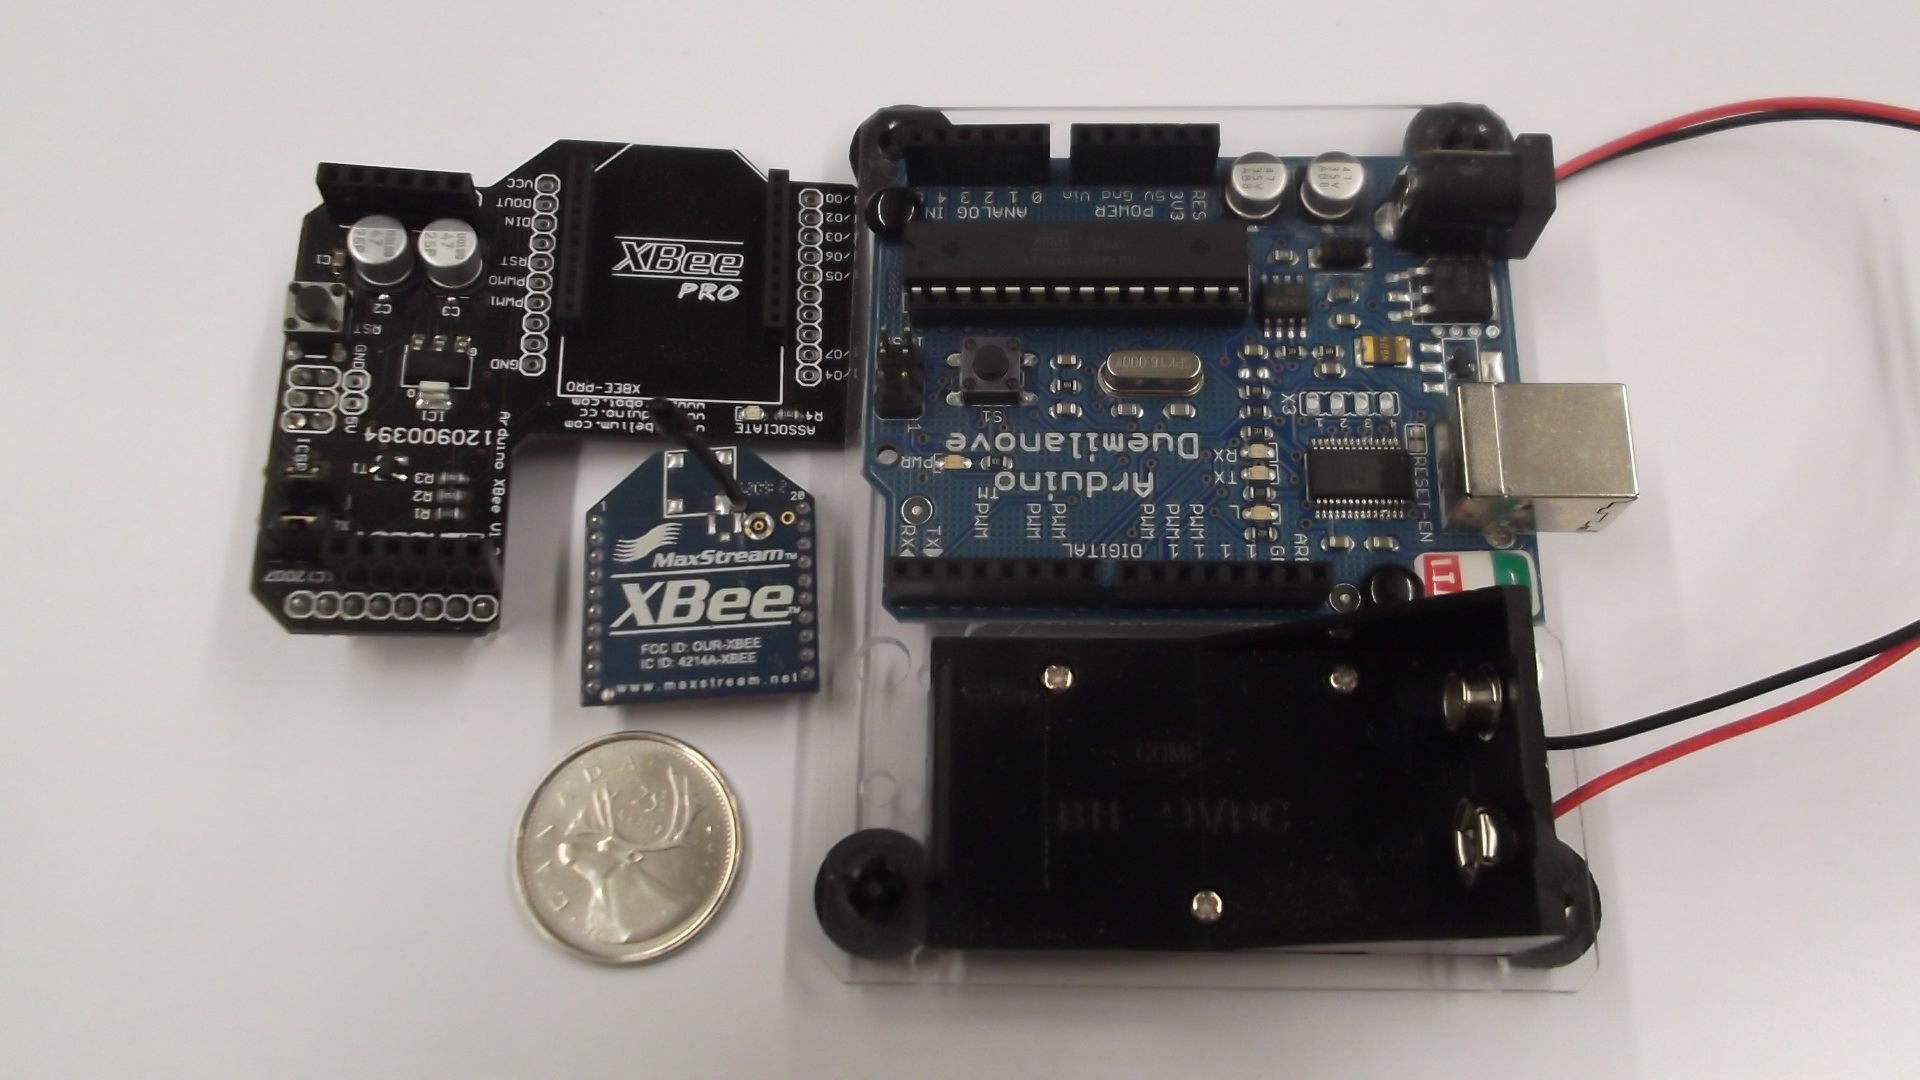
\includegraphics[height=3in]{images/motes/arduinoUnstack.jpg}
		\caption{The parts used to make the Arduino mote.}
		\label{fig:images_motes_arduinoStack}
	\end{figure}
	
	
	\paragraph{Possible modifications to the Stalker.}
    
    There is no battery packaged with the Arduino Duemilanove, so adding a battery is 
    necessary for the mote to work in the network. The Duemilanove is a custom 
    setup, and could be considered to be a heterogeneous mote by design.
    
    The Stalker ships with a button-cell battery that would not provide the stalker 
    with a very long lifespan. A larger battery would be necessary to make the Stalker 
    a useful mote.
		

	\paragraph{\emph{Uses for the Stalker and Arduino in a Heterogeneous WSN.}}
	
	The Stalker could be used for a routing mote, utilizing it's large
	storage capabilities provided by the MicroSD card. The Stalker could 
	also be used as a customized sensing node, using an Arduino-compatible 
	shield, or by using the Stalker's general purpose pins to connect to a sensor.
	
	\paragraph{\emph{Software used.}}
	
	Since the Stalker does not have a radio built onto the board, a third-party
	radio must be used. The Stalker provides an XBee-compatible port to host a radio.
	This XBee-compatible port uses the serial port on the Stalker board to contact the 
	radio. This works well with XBee radios, as they natively work in `transparent mode', which 
	means that the serial transmissions are sent over-the-air to other XBee radios
	in a way that the software using the radio need not know that a radio is being used.
	
	Since this project requires developing custom packets, a different mode must be used 
	when using the XBee radios to send and receive custom packets. The XBee Series 2, which
	is used in the experiment, has a mode called `API mode', that allows a developer to 
	create and read packets manually. A library named Arduino-Xbee~\cite{xbee-arduino} was 
	used to create and parse 802.15.4 packets properly. The library was modified to be
	more flexible and configureable to be more useful in the experiments.

\subsubsection {tMote Sky}
	The origins of the tMote Sky are from University of California, Berkeley. The basic 
	design is named Telos~\cite{telosOriginalPaper}, and has been marketed by several
	companies. The Telos mote was marketed by MoteIV, renaming it the tMote Sky.  
	MoteIV has been rebranded and renamed Sentilla. Sentill is still marketing the motes, as the Sentilla Mica.
	The motes have also been marketed as Crossbow, renamed to JCreate, all of which have a 
	similar design as seen in Figure~\ref{fig:images_motes_tmoteOneSide}.
	Each of these rebranded Telos motes have slightly different processors with 
	slightly differing memory sizes and sensors. The Telos variants are therefore 
	heterogeneous due to all of the different variants that are available.

	
	\paragraph{\emph{Possible modifications to the tMote Sky.}}
	The Telos mote has a large built-on power supply, and should not need a larger
	power supply. 
	The Telos does not have a large onboard memory, adding an external
	memory would make it a good router/clusterhead mote.
	
	%TODO - more? or move?
		
\begin{figure}[htbp]
	\centering
		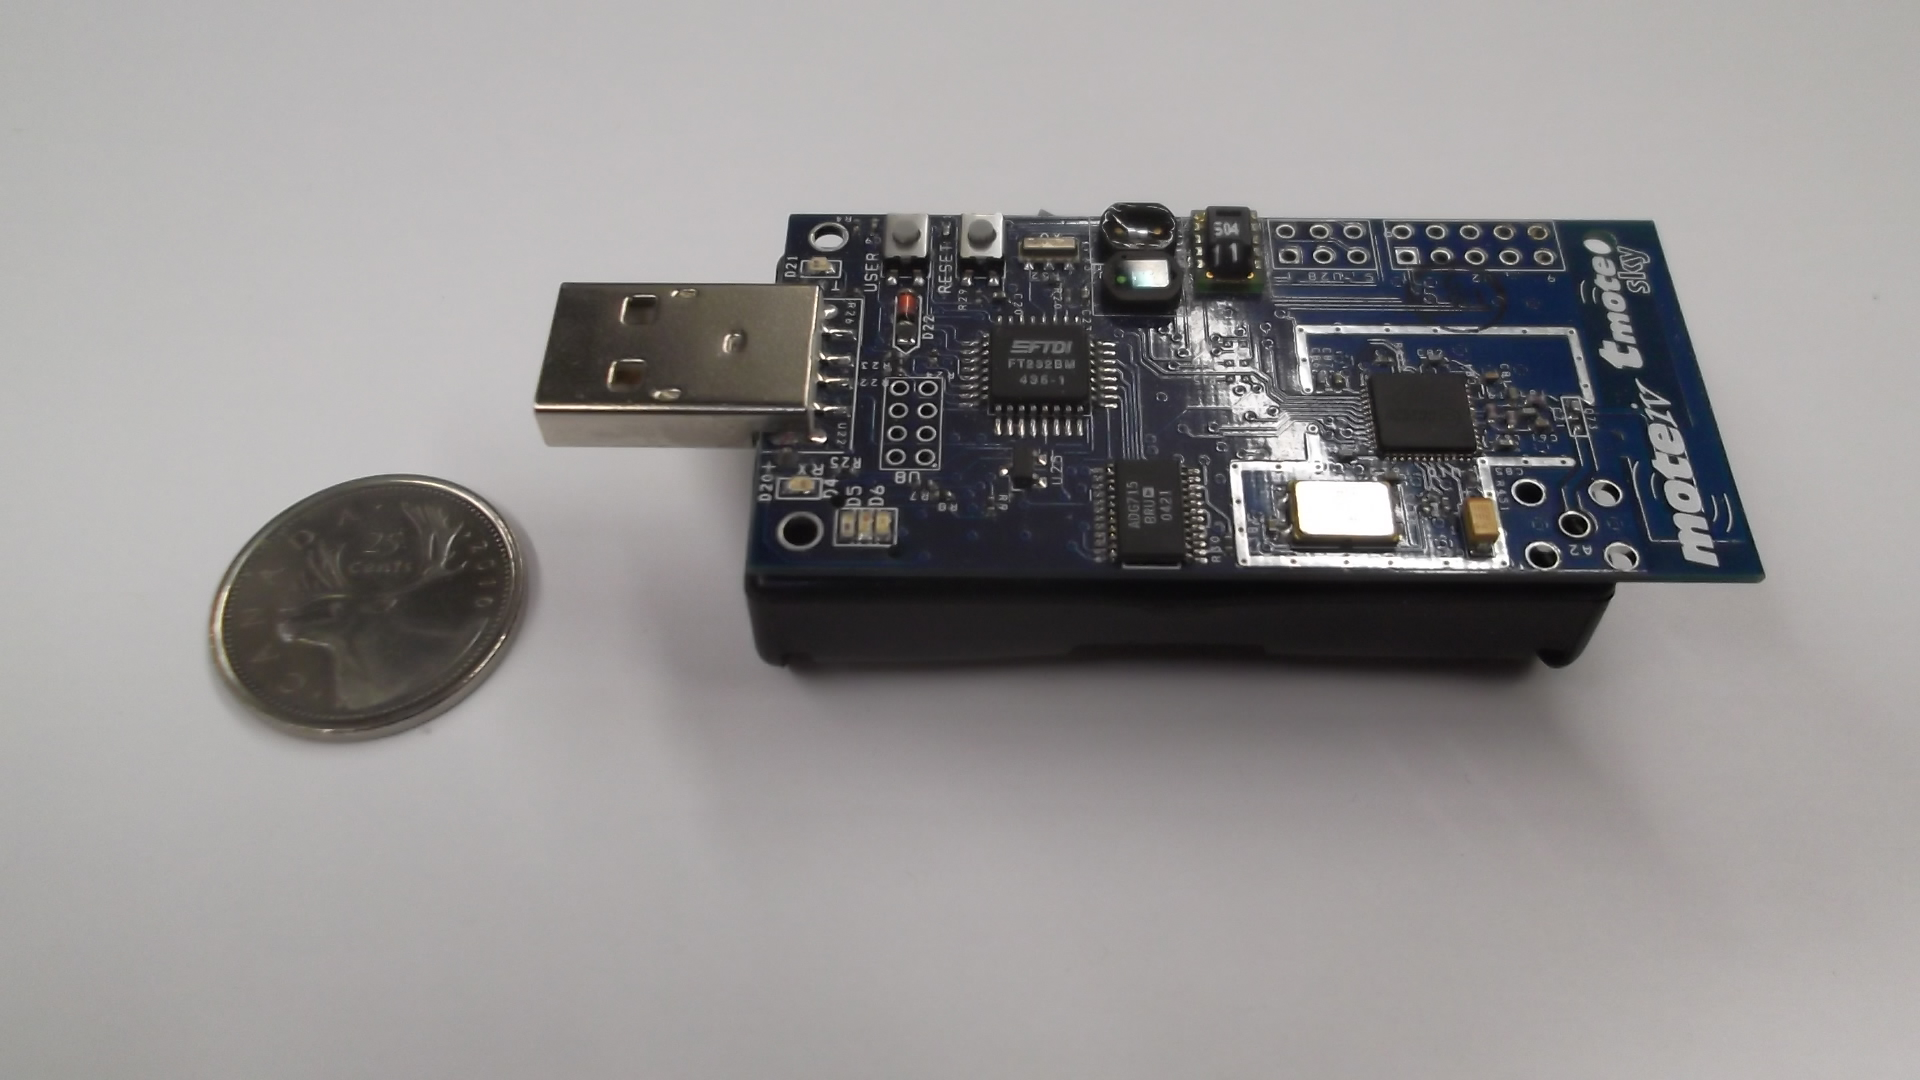
\includegraphics[height=3in]{images/motes/tmoteOneSide.jpg}
	\caption{The tmote Sky, which is a Telos variant.}
	\label{fig:images_motes_tmoteOneSide}
\end{figure}

	\paragraph{\emph{Uses for the tMote Sky in a Heterogeneous WSN.}}
	There are a number of onboard sensors making this a good mote for
	sensing tasks. Though, the large battery also makes the tMote a good candidate for 
	clusterhead, making the tMote a very versatile mote.
	

\subsection{Heterogeneous Setup of the Motes}	
Table~\ref{itsaTable} summarizes the motes, comparing the processors, radios, memory and battery power.
From the table it is easy to see the stark differences between the motes. The SunSPOT 
has a huge amount of memory and much more powerful processor than the
other motes, but its battery is tiny. The tMote has a
full operating system that is very easy to work with, and 
a large battery, but not a lot of flash memory. Though, the amount of flash memory is 
large in comparison with the Stalker and the Arduino which have almost no memory and very small extended memory.

Clearly, the SunSPOT is the most powerful mote in every respect except battery power. The tMote will take
the clusterhead head task the most frequently due to it's good extended memory size and battery power. The Stalker
and Arduino will not likely be clusterheads due to the limited extended memory which equates to limited 
queue sizes available on the devices.

While creating the testbed deployment, developing the  software for LEACH and HCCP on the 
Stalker was an issue, due to the very limited program space. Due to this, a minimalistic, chopped down
version of Contiki OS had to be made. The software uses the message queue code and interrupt callback code
from Contiki, while removing all other functions of the OS.
Contiki functions that were removed were any threads and context switching, drivers for sensors and  portability code 
so this version of Contiki can only run on Arduino microcontrollers.
This code was ported to the  Arduino with the ATmega 328 chip first, then an
even more stripped-down version had to be made for the Stalker with the less powerful ATmega 168p chip. 
The Stalker version of the software turns the
message queue into a ring buffer, and has limited roundtable abilities which only allow the Stalker to
accept routing information, and do nothing else during the Roundtable time.

Clearly, any of the modifications previously discussed could add more heterogeneity to this
already highly heterogeneous network if so desired.
	
\begin{table}
\begin{center}
\begin{scriptsizetabular}{|c|c|c|c|c|c|}
\hline
~ &  &  & & \textbf{Extended} & \textbf{OS /} \\
 & \textbf{Processor} & \textbf{Radio} &  \textbf{Memory} & \textbf{Memory} & \textbf{Software} \\
\hline
\textbf{SunSPOT} & 400 MHz 32-bit ARM920T & CC2420 & 1 MB & 8 MB & SunSPOT Framework \\
\hline
\textbf{tMote} & 8 MHz 16-bit TI MSP430 & CC2420 & 10 kB & 48 kB & Contiki OS \\
\hline
\textbf{Stalker} & 20 MHz 8-bit Atmel ATmega 168P & XBee Socket & 1 kB & 16 kB & Minimal Contiki OS \\
\hline
\textbf{Arduino} & 16 MHz 8-bit Atmel ATmega 328 & XBee Socket & 2 kB & 32 kB & Minimal Contiki OS \\
\hline

\end{scriptsizetabular}
\caption[Comparison of Motes in Testbed Deployment]{Comparison of Motes in Testbed Deployment.}
\label{itsaTable}
\end{center}
\end{table}
% http://arduino.cc/en/Main/ArduinoBoardDuemilanove/
% http://www.atmel.com/devices/atmega168p.aspx
% http://www.seeedstudio.com/wiki/Seeeduino_Stalker_v1.0
% http://www.sunspotworld.com/docs/index.html
% http://www.eecs.harvard.edu/~konrad/projects/shimmer/references/tmote-sky-datasheet.pdf
% 

\subsection{Testbed deployment}

To test the real-world feasibility of HCCP, a controlled physical deployment was run. 
SunSPOTs were used exclusively in the controlled deployment, as they were 
readily available in large quantities. A problem that plagued both  testbed deployments was that 
the SunSPOTs used were about five years old, and the rechargeable batteries that 
are built-in were starting to show signs of age. In the deployment, some of the motes
had the low battery warning light illuminated immediately despite being
fully charged. Due to the poor batteries, some of the motes
started dying after only 4 hours of running the experiment.
Due to the wear on the rechargeable batteries,
all the motes had a different amount of charge to use, which made the network
heterogeneous in terms of battery power. Adding different types of motes would
make the network more heterogenous, but the results would be very difficult to interpret due to the
amount of heterogeneity.



LEACH was set up as prescribed by Heinzelman et al.~\cite{leach} adding beacon routing information to the
Clusterhead Election announcement.

\subsubsection{House Monitoring Deployment}
\begin{figure}[htb]
    \centering
        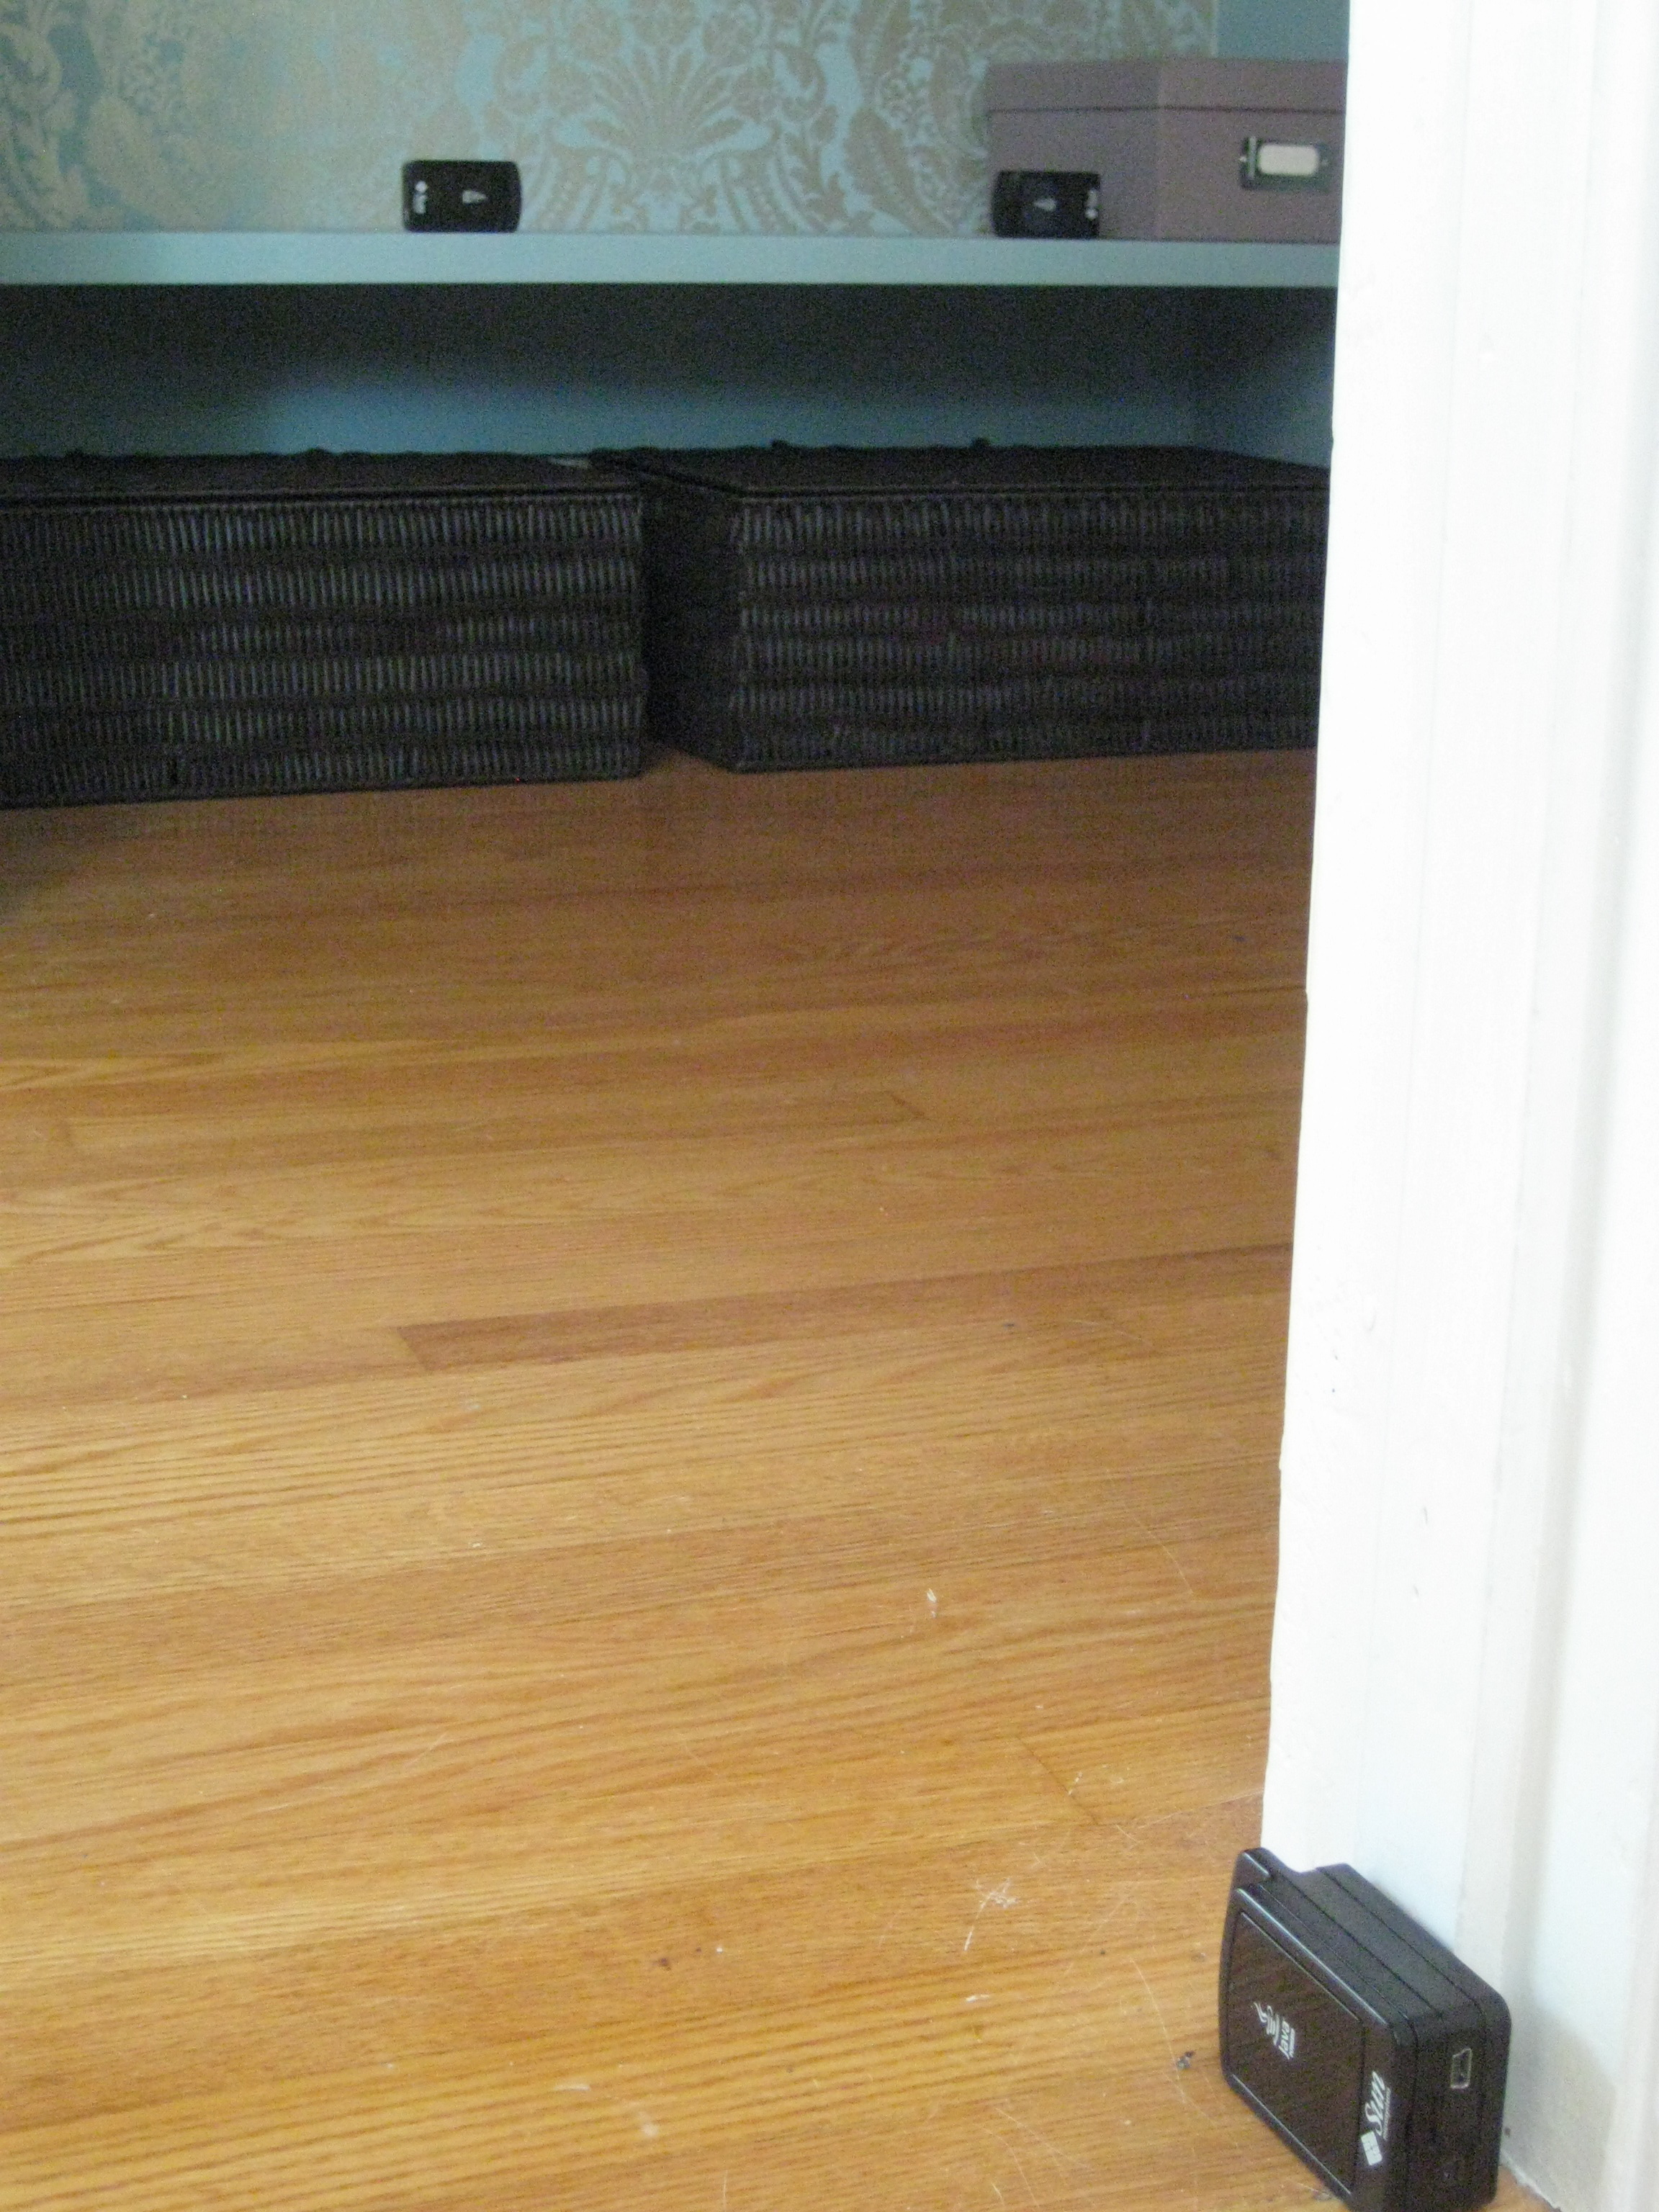
\includegraphics[height=5in]{images/deployment/hallway.JPG}
    \caption{Motes distributed around a house.}
    \label{fig:images_deployment_hallway}
\end{figure}

To show HCCP working in a real-world scenario, motes were distributed around a house.
Setting out motes around a house can simulate house monitoring for temperature, humidity
or even security. Motes could also be used in a house for home automation such as 
turning on lights in the room as a person enters, or having moving what's on television
from one room to the next as a person moves through a house.


The motes were deployed at various heights across a house as seen in Figure~\ref{fig:images_deployment_hallway}, with some motes placed outside
in waterproof containers. 
The networks had 44 motes and 1 sink distributed over (110) square meters (about 1200 square feet)
on various different levels and were made to communicate through various different materials.
The motes relayed their messages back to a sink that was placed centrally
in the house, this provided many routes back to the sink from any given mote. The motes were setup to create five new messages per minute, 
with all messages to be routed 
towards the sink.
Radio range was reduced to 4 meters line-of-sight to keep the network maintainable
and to ensure the network was a multi-hop network. Motes on the edges of the deployment were
setup to be at least three hops away.
The same network layout was used 
with both HCCP and LEACH deployments.


\begin{figure}[tb]
    \centering
        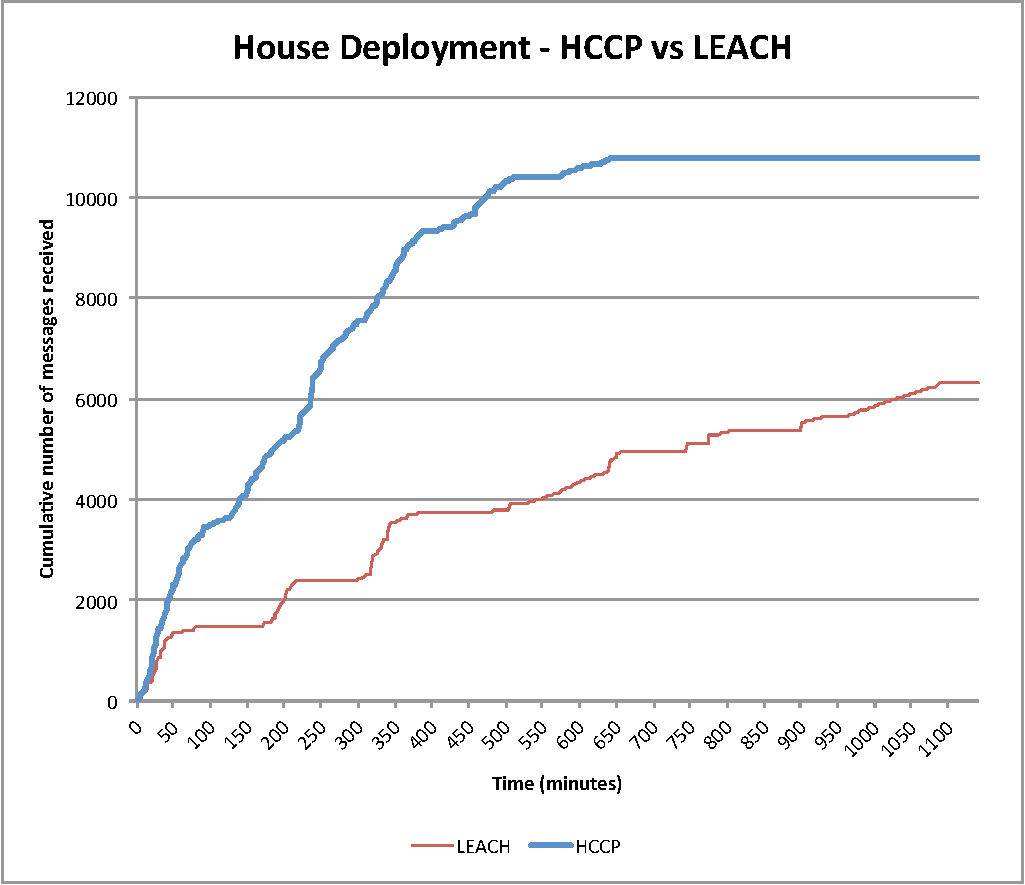
\includegraphics[width=5in]{images/deployment/houseResults.pdf}
    \caption{Cumulative number of messages received from the deployment done in a house.}
    \label{fig:images_deployment_houseResults}
\end{figure}

HCCP proved to be very effective at moving messages to the sink faster, as seen in Figure~\ref{fig:images_deployment_houseResults}.  
At 600 minutes (10 hours) the 
motes closest to the sink became inoperable, stopping the progress of the network.
Since the network was setup as quite sparsely,  a few motes dying early near the sink would have a large 
effect on the network. The performance of LEACH also degrades after the 600 minute mark, having received
62\% of its messages before the 10 hour mark.

Before the 10 hour mark, HCCP achieved approximately double the message throughput
that LEACH did. Also, HCCP had a much more consistent curve, creating a more linear chart. LEACH
has a step-function, probably due to the 5\% clusterhead rate as prescribed by Heinzelman et al.\ 
in their description of LEACH. Since the network cycle was setup to take one minute, messages can only 
flow into the motes next to the sink every 20 minutes, when the motes next to the sink choose to become clusterheads.

HCCP, on the other hand, was focused on Message Queue (95\%) and Battery Power (5\%). As the queues of the motes filled, 
they would be less likely to be clusterheads, allowing messages to to flow out of them. 
Then, as motes further away from the sink get full of messages, they 
are less likely to become clusterheads. As the motes further away
choose to be clusterheads less frequently, the motes close to the sink 
will more likely be clusterheads, which allows the messages flow 
towards the sink. As the motes close to the sink fill with messages from the motes further
from the also sink fill with messages, they will not be clusterheads as frequently, which
allows the messages to be sent to the sink.


\subsubsection{Grid Deployment}

\begin{figure}[htb]
    \centering
        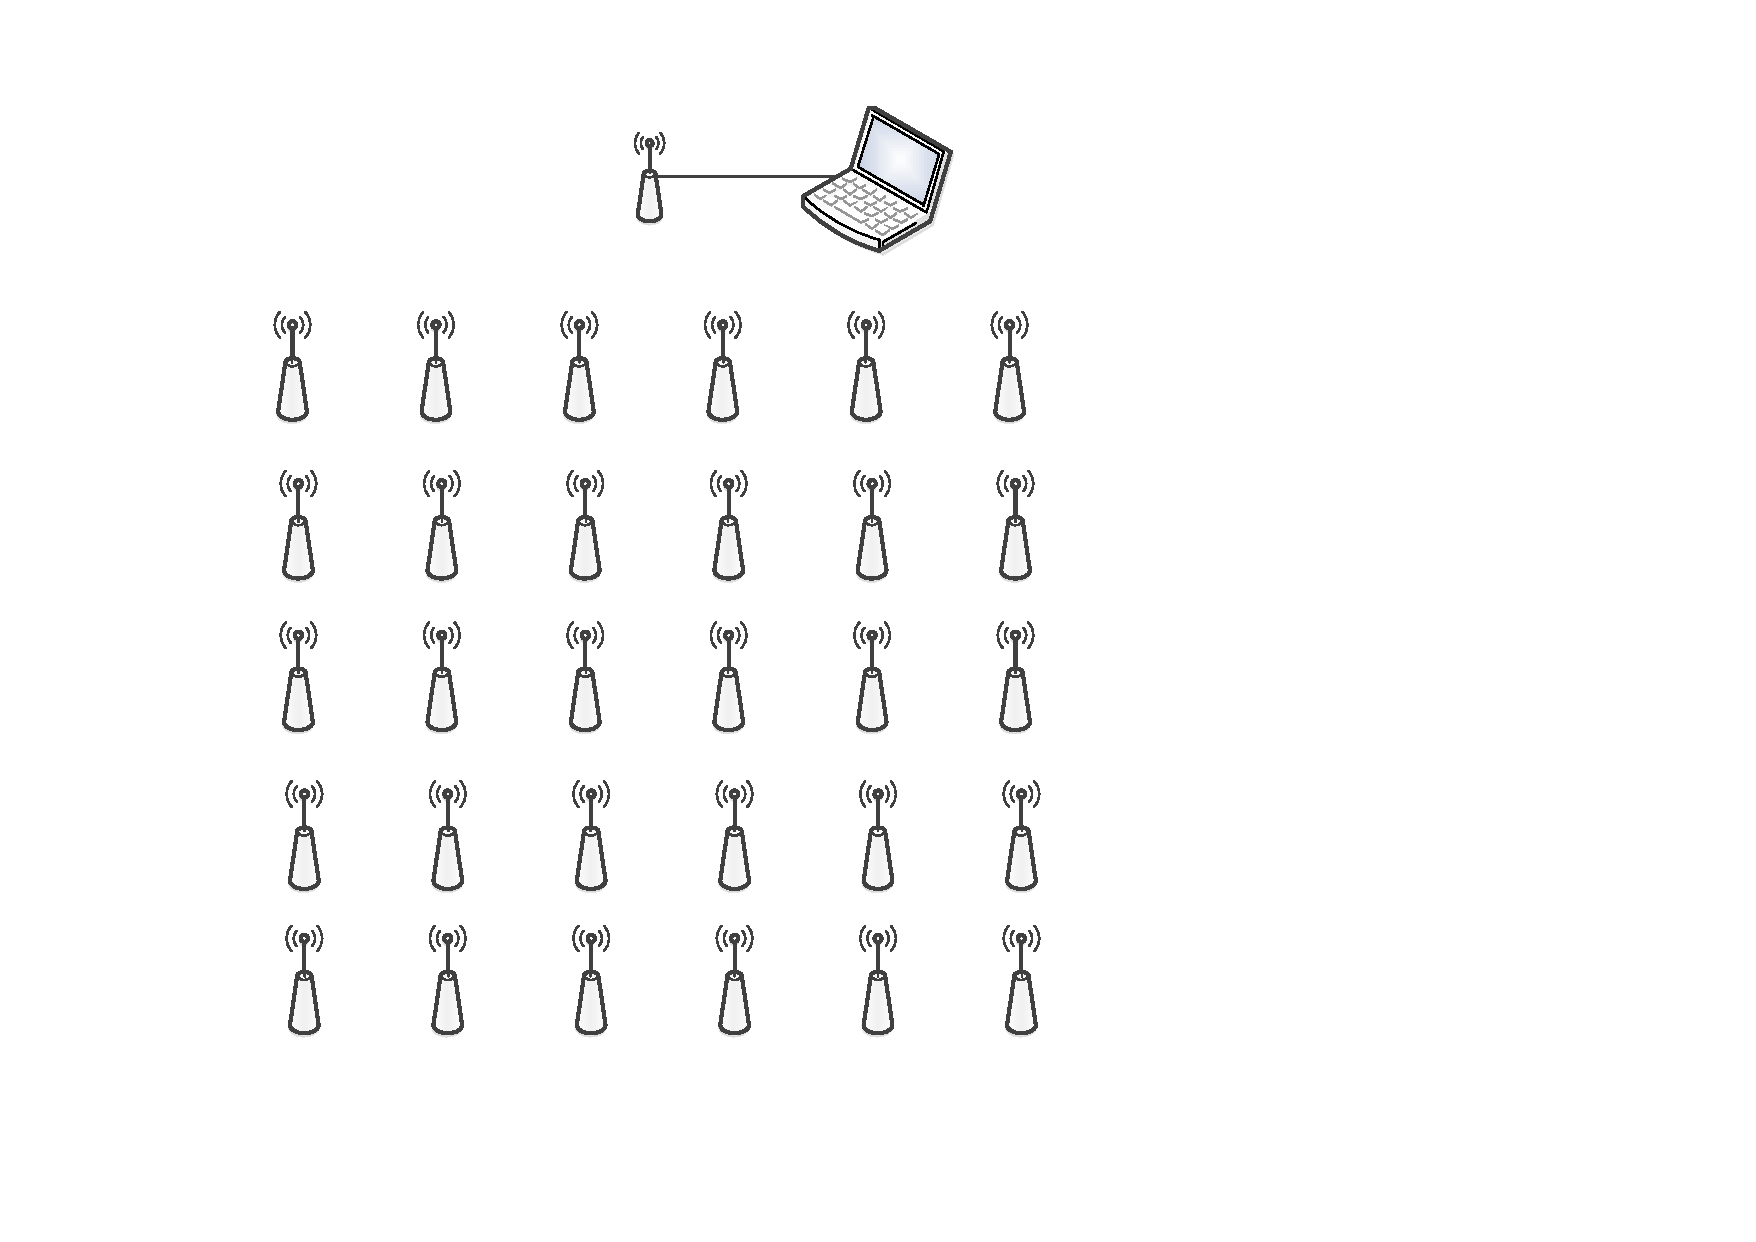
\includegraphics[height=3.5in]{images/deployment/gridChopped.pdf}
    \caption{The grid deployment setup.}
    \label{fig:images_deployment_gridChopped}
\end{figure}


A second deployment was done with 30 motes and a sink. The motes were set up in a 5 by 6 grid,
with 1.5 meter spacings between them. This made the grid spread out over a 7.5 meter by 9 meter 
area. The radio range was set to a 6 meter range, which will degrade over the lifespan of the network.
The sink was set up at the side of the network, as seen in Figure~\ref{fig:images_deployment_gridChopped}.

During both the LEACH and HCCP deployments, some of the motes immediately had the battery low warning light illuminated, 
despite the fact all batteries were fully charged before the deployment. Rechargeable batteries lose their ability to 
hold a charge as they age; since these are older motes it is only natural that some of the batteries would
be quite degraded. The motes that were nearly dead at time of deployment were left in the network for the test.

One problem about battery-powered devices is that as the battery drains, the device 
becomes unreliable. This unreliability stems from transistors not switching properly due
to not being able to draw enough current, or not having enough voltage to cause the
transistor to change state. Since the SunSPOT batteries were old, the motes were only reliable 
for about 10 hours. After 10 hours the motes could not maintain the network schedule, as 
the timer would not work properly. Interestingly, during the HCCP deployment, 
3 motes lasted over 60 hours but didn't send any messages during that time, meaning that the
motes were in deep sleep for that entire time. Not waking from sleep can happen when 
the wakeup timer never fires, leaving the mote asleep indefinitely.


\begin{figure}[tbh]
    \centering
        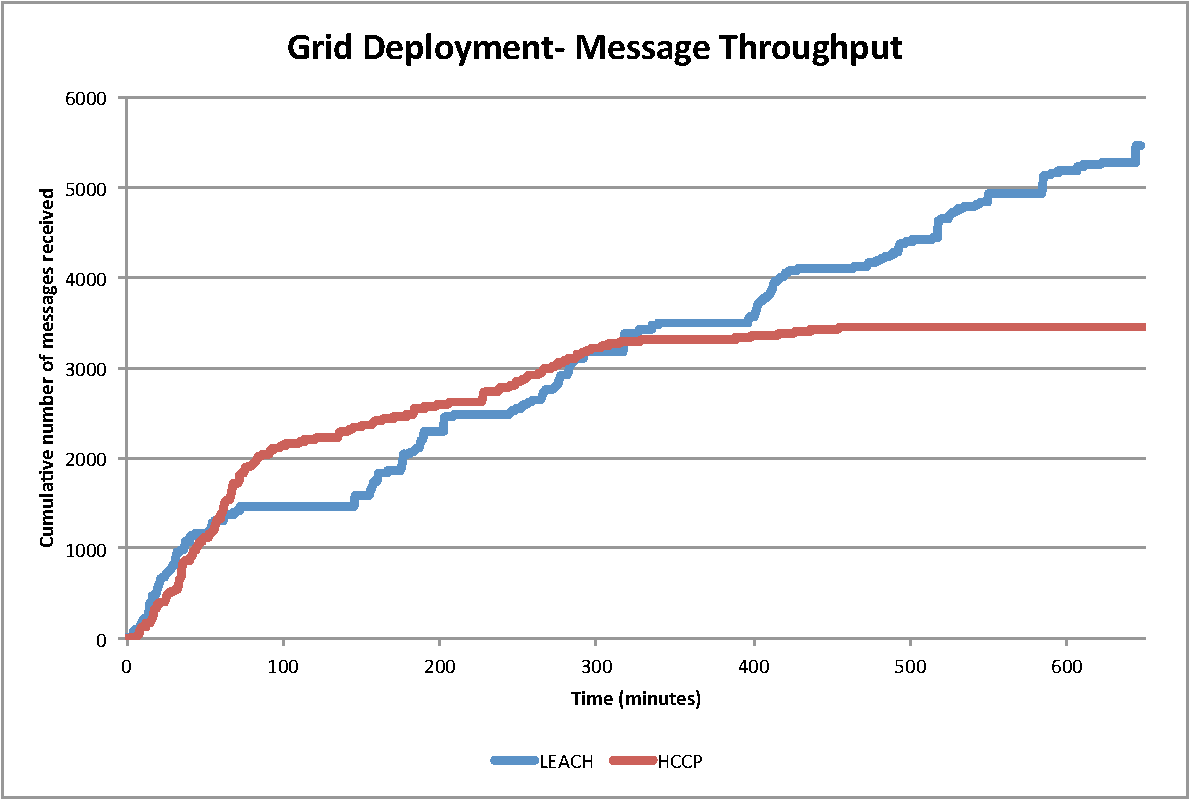
\includegraphics[height=3in]{images/deployment/results.pdf}
    \caption{Results from LEACH and HCCP Grid Deployments}
    \label{fig:images_deployment_results}
\end{figure}

The results from the grid deployment is shown in Figure~\ref{fig:images_deployment_results}.
At the start of the deployments, HCCP started with a better message throughput, as expected from
the results of the simulations. The throughput of HCCP then drops to a slower rate, allowing LEACH to 
catch up, and overtake it. HCCP then levels off, as motes begin to fail as the 300 minute (5 hour) point
approaches. Motes close to the sink were failing due to going to sleep, causing the messages to not have a
route to the sink.

The LEACH curve is more consistent than the HCCP curve, having steady steps. The
steps are quite interesting, as the LEACH network cycle was setup to take a minute, so the steps
should be in shorter cycles than 10 minutes.

If the motes had be provisioned with larger batteries, HCCP should maintain the slope it was forming before the 100 minute mark.
The HCCP deployment had the unfortunate luck of having the motes closest to the sink die first due to 
poor batteries, dying early of reasons unrelated to the protocol.

For network lifespan, the last message received in the LEACH network was at 646 minutes (10.75 hours). 
Since the motes closest to the sink in the HCCP deployment had problems waking from sleep, the 
last message was received at 3489 minutes (58.15 hours). This huge network lifespan is due to 
a mote rebooting after being in deep sleep for a long time, rejoining the network and sending it's 
messages to the sink. LEACH likely had motes do the same thing, but the motes weren't as close to the sink
and therefore did not create these odd data points.


Overall, HCCP has worked as a proof-of-concept in a real-world deployment. Since older motes were 
used, the results are difficult to interpret. Despite these difficulties, HCCP worked 
well, showing its real-world plausibility.
 




